\chapter{Arquitectura de VirtShell}
\label{Arquitectura}

En este capítulo se introduce y elabora la arquitectura de VirtShell, se mencionan los elementos arquitectónicos mas significativos que se tuvieron en cuenta en la elección de los módulos necesarios para interactuar con el sistema y las relaciones entre ellos. Adicionalmente se describen las características que gracias a la arquitectura planteada permite el framework. Por ultimo, se mencionan brevemente los diferentes módulos y sus funciones mas importantes.\\
\\
VirtShell Framework es concebido como una plataforma que proporciona herramientas para la automatización y gestión de infraestructura, facilitando tareas como la creación, despliegue, mantenimiento y monitoreo tanto de recursos virtuales como físicos vía web. Así mismo, es pensada para que cualquier desarrollo de software con acceso a Internet (sitio web, aplicación móvil, etc.) pueda interactuar con la infraestructura virtual tan solo consumiendo un API de Internet.\\
\\
Las motivaciones mencionadas conducen a los requisitos para una arquitectura destinada a separar claramente responsabilidades, usando protocolos abiertos, modificables, escalables, y al mismo tiempo adecuado para la creación rápida de nuevas acciones. \\
\\
En la búsqueda del adecuado estilo arquitectural para el API de VirtShell, se evaluaron dos estilos de servicios web: el estilo \emph{Remote Procedure Call} (RPC) y el estilo arquitectural REST (\emph{Representational State Transfer}) \cite{fielding00}. La evaluación dio como resultado que el estilo arquitectural que mejor se acomodaba a los requisitos planteados era el estilo arquitectural REST, debido a que es un estilo nativo del Web, lo que hace que la información disponible esta regida por las mismas normas que rigen los sitios web, ademas, el estilo ofrece mejor escalabilidad, acoplamiento y rendimiento. Un detallado comparativo entre los dos estilos se encuentra en \cite{Xinyang09}. A continuación se muestran a grandes rasgos las diferencias entre ambos estilos y razones adicionales para la preferir el estilo REST.

\section{RPC}
RPC se caracteriza generalmente como un único URI \footnote{URI es una cadena de caracteres que identifica los recursos de una red de forma unívoca} a través del protocolo HTTP en el que se pueden llamar muchas operaciones, por lo general solo se usan las operaciones GET y POST. Cuando se pasa una solicitud estructurada, esta incluye el nombre de la operación a invocar y los argumentos que desea pasar a la operación; la respuesta será devuelta también en un formato estructurado.\\
\\
Una cosa a tener en cuenta es que por lo general RPC hace todo el informe de errores en el cuerpo de la respuesta; el código de estado HTTP no variará, lo que significa que hay que fijarse en el valor de retorno para determinar si se ha producido un error.\\
\\
Muchas implementaciones de RPC también proporcionan documentación para sus usuarios finales a través del protocolo en sí. Por ejemplo para SOAP \footnote{SOAP es un protocolo estándar que define cómo dos objetos en diferentes procesos pueden comunicarse por medio de intercambio de datos XML.} lo hace a través del WSDL \footnote{WSDL es un formato XML que se utiliza para describir servicios Web.}. Esta característica de auto-documentado puede proporcionar información muy valiosa para el consumidor sobre cómo interactuar con el servicio.\\
\\
En resumen, los puntos a tener en cuenta acerca de RPC son:

\begin{itemize}
\item Un extremo de servicio, muchas operaciones.
\item Un extremo de servicio, un método HTTP (normalmente POST).
\item Formato de solicitud predecible estructurada, formato de respuesta estructurada y predecible.
\item Formato de informe de errores predecibles estructurada.
\item Documentación estructurada de operaciones disponibles.
\end{itemize}

\vspace{5mm}

Dicho todo esto, RPC es a menudo un mala elección para hacer APIs web porque:

\vspace{5mm}

\begin{itemize}
\item No se puede determinar a través de la URI la disponibilidad de varios recursos.
\item Falta de almacenamiento en caché de HTTP
\item La imposibilidad de usar verbos HTTP nativos para operaciones comunes 
\item Falta de códigos de respuesta, se requiere la introspección de los resultados para determinar si se ha producido un error.
\item Los clientes no podrán consumir formatos de serialización alternativos.
\item Los formatos de mensajes a menudo imponen restricciones innecesarias sobre los tipos de datos que se pueden enviar o devolver.
\end{itemize}

\vspace{5mm}

En pocas palabras, RPC no utiliza las capacidades completas del protocolo HTTP.

\section{REST}
REST es un estilo de arquitectura de software que proporciona un enfoque practico y consistente para solicitar y modificar datos en torno a la especificación del protocolo HTTP. \\
\\
El termino REST es la abreviatura para ``Representational State Transfer.", el cual aprovecha las fortalezas de los protocolos HTTP y HTTPS \footnote{HTTPS, es un protocolo de aplicación basado en el protocolo HTTP, destinado a la transferencia segura de datos de Hipertexto, es decir, es la versión segura de HTTP.}. Un buen API REST debe constar de:

\begin{itemize}
\item Usar URIs como identificadores únicos de los recursos.
\item Aprovechar el espectro completo de verbos HTTP para las operaciones sobre los recursos.
\item Permitir el manejo de varios formatos de representación de recursos.
\item Proporcionar vinculación entre los recursos para indicar las relaciones. (Por ejemplo, enlaces hipermedia, como los encontrados en los antiguos documentos HTML plano)
\end{itemize}

Todo esta teoría dice cómo deben actuar los servicios REST, pero dice muy poco acerca de la forma de implementarlos. REST es más una consideración arquitectónica; sin embargo, esto significa que al momento de diseñar un API REST se debe considerar muchas opciones, algunas como que formato se va a exponer, como se reportaran los errores, como se comunicara los métodos HTTP disponibles, como se manejaran características de autenticación, como se suministraran las credenciales en cada petición, etc.\\
\\
En pocas palabras, un API REST proporciona una increíble flexibilidad y potencia, pero requiere de tomar muchas decisiones con el fin de proporcionar una sólida experiencia y calidad para los consumidores.

\section{Características}
VirtShell es un framework de código abierto y bajo la licencia BSD, que permite utilizarlo para proyectos de cualquier tipo, incluso comerciales, sus características principales son: 

\begin{description}
\item [Programable] VirtShell esta orientado a realizar el aprovisionamiento de sus instancias principalmente por medio de scripts escritos en shell, permitiendo aprovechar todas las estructuras y utilidades del lenguaje de programación. Sin embargo, el lenguaje de shell no es de uso obligatorio, el  método de aprovisionamiento puede ser el de la preferencia del usuario. 
\item [Repetible] VirtShell ofrece herramientas para que los scritps de aprovisionamiento sean configurables y  puedan ser ejecutados varias veces en diferentes ambientes de desarrollo o producción.
\item [Modular] VirtShell es un framework organizado de forma modular. Los módulos se encuentran agrupados en categorías que ofrecen las herramientas necesarias para la administración y aprovisionamiento de múltiples recursos virtuales. De igual manera y dada las características de REST, los módulos están diseñados para que se puedan dividir en diferentes servidores obteniendo "micro APIs", lo que permite dividir los procesos y atender diferentes tipos de operaciones del API. 
\item [Seguro] VirtShell provee varias capacidades y servicios para aumentar la privacidad y el control de acceso a los diferentes recursos. Los servicios de seguridad permiten crear redes y controlar el acceso a las instancias creadas, así como definir y administrar políticas de acceso a usuarios y permisos sobre cualquier recurso del sistema como por ejemplo scripts de creación y aprovisionamiento.
\item [Extensible] Al ser VirtShell de código abierto, el API puede modificarse, crecer fácilmente y versionarse de diferentes maneras. Adicionalmente, VirtShell fue diseñado con la idea de cargar código dinámicamente, permitiendo extender el comportamiento del framework agregando plugins en tiempo de ejecución.  Asi mismo, VirtShell permite extender el comportamiento del shell desplegando comandos propios que proporcionan ahorro en tiempo y en complejidad.
\item [Inyección de dependencias virtuales] VirtShell adopta la idea del patrón de Inyección de Dependencias \footnote{es un patrón de diseño orientado a objetos, en el que se suministran objetos a una clase en lugar de ser la propia clase quien cree el objeto. El término fue acuñado por primera vez por Martin Fowler.} \cite{fowler04} para conseguir scripts de aprovisionamiento mas desacoplados. De esta manera facilita la configuración de las dependencias que tiene un recurso virtual de otras máquinas virtuales. Para ello, el framework permite declarar el listado de dependencias de recursos virtuales que tiene un script de aprovisionamiento encargándose del correcto acople entre los diferentes recursos virtuales.
\item [Interoperable] Al seguir el estilo arquitectónico REST y contar con la documentación detallada sobre cada uno de los recursos y urls que expone el API de VirtShell, se logra una capacidad clave para la administración remota de la infraestructura virtual. Esta capacidad se refiere al hecho de poder desarrollar aplicaciones en cualquier plataforma y para cualquier dispositivo electrónico, lo que permite funcionar con otros productos o sistemas existentes o futuros.

\end{description}

\section{Módulos}
VirtShell Framework consiste de características organizadas en 13 módulos. Estos módulos son agrupados en Seguridad, Administración y Aprovisionamiento. Estos elementos se usan de manera separada pero trabajan juntos para proveer la información necesaria para que los agentes realicen su trabajo en los hosts que albergaran los recursos virtuales, como se muestra en la figura \ref{fig:framework}. \\

\begin{figure}[h]
    \centering
	\caption{Visión general del framework de VirtShell}
	\label{fig:framework}
	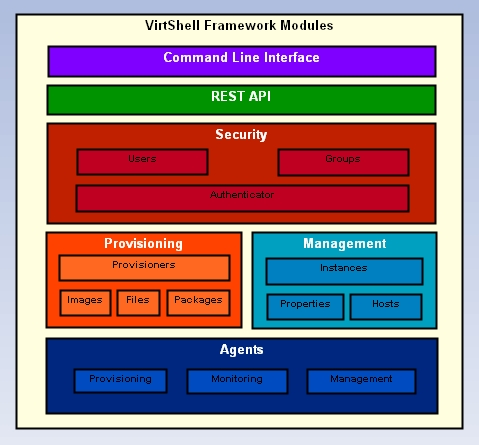
\includegraphics[width = 0.8\textwidth]{../architecture/v1/diagrams/framework}
\end{figure}

Las siguientes secciones detallan los módulos disponibles para cada característica. 

\subsection{Security}
Seguridad consiste de los módulos de \emph{users} (usuarios), \emph{groups} (grupos) y el modulo \emph{authenticator} (de autenticación). El control de los usuarios y grupos son elementos clave en la administración del framework. Los \textbf{Usuarios} pueden ser personas reales, es decir, cuentas ligadas a un usuario físico en particular o cuentas que existen para ser usadas por aplicaciones específicas. \\
\\
Los \textbf{Grupos} son expresiones lógicas de organización, reuniendo usuarios para un propósito común. Los usuarios dentro de un mismo grupo pueden leer, escribir o ejecutar los recursos que pertenecen a ese grupo.\\
\\
El módulo de \textbf{autenticación} soporta el proceso por el cual cuando un usuario se presenta a la aplicación puede validar su identidad. Este módulo es quien decide0 si el usuario tiene permiso para ingresar al sistema y el nivel de acceso a un recurso dado. En el capitulo 4 se detalla el proceso de autenticación y autorización.

\subsection{Managment}
Administración consiste de los modulos \emph{hosts} (anfitriónes), \emph{partitions} (particiones), \emph{enviroments} (ambientes), \emph{instances} (instancias), \emph{properties} (propiedades) y \emph{tasks} (tareas). \\
\\
El módulo de \textbf{anfitriónes} lleva registro de nodos físicos, servidores o máquinas virtuales, que se encuentren conectados a la red y que permitan albergar instancias virtuales. Los anfitriónes son clasificados de acuerdo a diferentes combinaciones de CPU, memoria, almacenamiento y capacidad de trabajo en red, dando flexibilidad para elegir la opcion mas adecuada para las necesidades de las aplicaciones destino. En otras palabras el tipo de anfitrión determina el hardware del nodo físico que sera usado por los recursos virtuales.\\
\\
El módulo de \textbf{particiones} permite dividir los anfitriones en secciones aisladas de disponibilidad. Cada partición puede ser usada para definir áreas geográficas separadas o simplemente para dividir los nodos físicos en subgrupos destinados a diferentes usos o equipos de trabajo o tipos de clientes.\\
\\
El módulo de \textbf{ambientes} permite dividir lógicamente una partición en subredes de trabajo más pequeñas, con lo que se crean grupos más pequeños con diferentes fines. En los ambientes de trabajo se configuran los usuarios que tienen permiso para interactuar trabajar con el.\\
\\
El módulo de \textbf{instancias} es un recurso virtual o máquina virtual o contenedor con parámetros y capacidades definidas en la cual se puede instalar el software deseado. Un usuario puede crear, aprovisionar, actualizar y finalizar instancias en VirtShell tanto como necesite dando la sensación de elasticidad \footnote{La elasticidad es una de las propiedades fundamentales de la nube. La elasticidad consiste en la potencia de escalar los recursos informáticos ampliándolos y reduciéndolos dinámicamente.} de la red.\\
\\
El módulo de \textbf{propiedades} permite consultar información de sistema, de las instancias o de los anfitriones físicos. La información que puede ser consultada es toda aquella que el sistema tenga disponible o que se pueda consultar por medio de comandos de sistema o comandos propios de VirtShell. Ejemplos de información que se puede consultar por medio de las propiedades es porcentajes de memoria y cpu usada, numero de procesos en ejecución, etc. Las propiedades pueden ser consultadas en una sola maquina, o simultáneamente en varias maquinas, o a un conjunto de maquinas de acuerdo a prefijos en su nombre.\\
\\
Finalmente, el módulo de \textbf{tareas} da la información y estado sobre las diferentes tareas o trabajos ejecutados en el sistema. Debido a que el medio para interactuar con los módulos de VirtShell es a través de un API REST, una petición de creación de un nuevo recurso virtual, puede ser largo si el aprovisionamiento involucra varias maquinas. Para evitar, tener una petición esperando respuesta, VirtShell crea una tarea que sera ejecutada de manera asincrónica, dando como respuesta, un identificador de la tarea, para que esta pueda ser consultada posteriormente y conocer el estado de la petición.


\subsection{Provisioning}
Aprovisionamiento consiste de los módulos \emph{provisioners} (aprovisonadores), \emph{images} (imágenes), \emph{files} (archivos) y \emph{packages} (paquetes).\\
\\
El módulo de \textbf{aprovisionadores} define un marco de aprovisionamiento de un recurso virtual y contiene las configuraciones necesarias para apoyar ese marco. La configuración fundamental de un aprovisionador, es la ruta del repositorio git \footnote{git es un software de control de versiones diseñado por Linus Torvalds}, donde se encuentran los scripts y archivos necesarios para realizar el aprovisionamiento. Del mismo modo la forma de ejecutar los scripts, hace parte de la configuración básica. Para ser mas ligero a VirtShell, los scripts de aprovisionamiento, deben estar registrados en un repositorio git público. VirtShell se encarga de descargar el repositorio y de ejecutar los scripts de aprovisionamiento, de acuerdo a la configuración especificada. \\
\\
Adicionalmente, los aprovisonadores cuentan con una manera de especificar las dependencias del nuevo recurso virtual. VirtShell se encarga de resolver las dependencias antes de realizar el aprovisionamiento del nuevo recurso, a su vez, suministra información de ellas a los scripts de aprovisionamiento si estos lo requieren. \\
\\
VirtShell utiliza como lenguaje de referencia, para la creación de scripts de aprovisionamiento, el lenguaje shell. Este cuenta con los recursos suficientes para interactuar con los diferentes sistemas operativos de las instancias. Sin embargo estos comandos se pueden extender usando el paquete de comandos propios de VirtShell, los cuales pueden abstraer muchas de las operaciones del shell. Esto facilita la escritura de los mismos o permite hacerlos independientes del sistema operativo en el cual van a ejecutarse.\\
\\
El módulo de \textbf{imágenes} proporciona la información necesaria de las imágenes que se encuentran registradas en el sistema. Cada vez que se crea un nuevo recurso virtual en un anfitrión, se especifica el nombre de la imagen almacenada en el sistema que sera usada, de una de las que se encuentra en el sistema. \\
\\
Las imágenes que se manejan en VirtShell son de dos tipos: ISO \footnote{Una imagen ISO es un archivo informático donde se almacena una copia o imagen exacta de un sistema de archivos o ficheros de un disco óptico, normalmente un disco compacto (CD) o un disco versátil digital (DVD).} y para contenedores. Las de tipo ISO, se encuentran guardadas en el repositorio de VirtShell, y su uso se enfoca a maquinas virtuales que interactuan con hypervisors. Las imágenes de tipo contenedor, se emplean para tecnologías de visualización de sistema operativo como LXC \footnote{LXC (Linux Containers) es una tecnología de virtualización a nivel de sistema operativo (SO) para Linux. } \cite{lxc16} y Docker \footnote{Docker es un proyecto de código abierto que automatiza el despliegue de aplicaciones dentro de contenedores de software, proporcionando una capa adicional de abstracción y automatización de Virtualización a nivel de sistema operativo en Linux.} \cite{docker16}. Estas son descargadas automáticamente de los repositorios de dominio público de los diferentes proveedores. \\
\\
El módulo de imágenes cuenta también, con la característica de crear automáticamente nuevas imágenes de tipo ISO a partir de las \emph{releases} (liberaciones) base de las diferentes distribuciones de sistemas operativos linux. Una vez creada la nueva ISO esta sera guardada en el repositorio interno para su posterior uso.\\
\\
El módulo de \textbf{archivos} proporciona una manera de almacenar archivos en VirtShell, los cuales pueden ser usados para almacenar 

El módulo de \textbf{archivos} proporciona una manera de almacenar archivos en VirtShell, los cuales pueden ser usados para almacenar información necesaria para crear imágenes o para enviarlos a uno o mas recursos virtuales de manera simultánea en un directorio especificado. Adicionalmente, permite especificar los permisos que tendrán los archivos.\\
\\
El módulo de \textbf{paquetes} facilita realizar funciones tales como la instalación de nuevos paquetes de software y actualización de paquetes existentes en uno o mas recursos virtuales de manera simultanea.


\subsection{Agents}
Los Agentes son servicios que se ejecutan localmente en cada anfitrión, y que se encuentra bajo la gestión de VirtShell. Estos son instalados y configurados en cada anfitrión de manera automática. Los agentes actúan con un cierto grado de autonomía con el fin de completar tareas en nombre del servidor.\\
